\chapter{磁铁}\label{ch:g1:magnets}

冰箱门上，几个小人儿举着图画，
不用胶水，不用胶带，也不用挂钩。拔下一个，背面毫无黏性 ---
可它却弹回去，牢牢吸住。
这些小人儿里都藏着一块磁铁。磁铁大有奇妙之处，
值得用整整一章的实验去探索。

\section{磁铁能吸住什么}

\begin{definition}[磁铁]\label{def:g1:magnets:magnet}
\emph{磁铁}\index{磁铁}是一种特殊的石块或金属，
它不必接触，就能把某些东西吸向自己。
磁铁会\emph{吸引}\index{吸引}它们。被它吸引的东西会贴上来；
其余的则对它毫不在意。
\end{definition}

\begin{example}[动手试一试：抓取测试]\label{ex:g1:magnets:test}
拿着磁铁在家里走一走，逐一试试：回形针、
钉子、冰箱门、木勺、塑料积木、
一张纸、玻璃杯、软木塞。磁铁能吸住回形针、
钉子和冰箱门 --- 对其余的东西一概不理。
只有一部分东西会被磁铁吸引。
\end{example}

\begin{omfigure}
\begin{tikzpicture}[scale=0.85]
  % bar magnet, two colored ends
  \draw[thick, fill=red!70] (0.2,1.15) rectangle (0.95,1.85);
  \draw[thick, fill=blue!60] (0.95,1.15) rectangle (1.7,1.85);
  \node[below, font=\small] at (0.95,1.0) {磁铁};
  % paperclip, rushing in
  \begin{scope}[shift={(2.75,2.0)}]
    \draw[thick, rounded corners=2.6pt]
      (0,0) -- (1.1,0) -- (1.1,0.42) -- (0.12,0.42) -- (0.12,0.14)
      -- (0.95,0.14) -- (0.95,0.30) -- (0.30,0.30);
  \end{scope}
  \draw[-Stealth, very thick, omThm] (2.6,1.95) -- (1.95,1.85);
  \node[right, font=\small] at (4.1,2.2) {回形针：吸住了！};
  % nail, rushing in
  \begin{scope}[shift={(2.55,0.55)}]
    \draw[thick, fill=omExo!35] (0,0.16) -- (0.4,0.06) -- (1.5,0.06)
      -- (1.5,0.26) -- (0.4,0.26) -- cycle;
    \draw[thick, fill=omExo!55] (1.5,-0.02) rectangle (1.62,0.34);
  \end{scope}
  \draw[-Stealth, very thick, omThm] (2.4,0.85) -- (1.85,1.05);
  \node[right, font=\small] at (4.35,0.7) {钉子：吸住了！};
  % cork, not interested
  \begin{scope}[shift={(8.3,1.55)}]
    \draw[thick, fill=brown!40] (0,0) -- (0.07,0.62) -- (0.63,0.62)
      -- (0.7,0) -- cycle;
    \draw[thick, fill=brown!25] (0.35,0.62) ellipse (0.28 and 0.09);
  \end{scope}
  \node[right, font=\small] at (9.35,1.85) {软木塞：无动于衷};
  % plastic brick, not interested
  \begin{scope}[shift={(8.2,0.3)}]
    \draw[thick, fill=yellow!70] (0,0) rectangle (1.0,0.5);
    \draw[thick, fill=yellow!50] (0,0.5) -- (0.25,0.72) -- (1.25,0.72)
      -- (1.0,0.5) -- cycle;
    \draw[thick, fill=yellow!45] (1.0,0) -- (1.25,0.22) -- (1.25,0.72)
      -- (1.0,0.5) -- cycle;
    \draw[thick, fill=yellow!80] (0.42,0.61) ellipse (0.13 and 0.055);
    \draw[thick, fill=yellow!80] (0.86,0.61) ellipse (0.13 and 0.055);
  \end{scope}
  \node[right, font=\small] at (9.7,0.55) {塑料积木：};
  \node[right, font=\small] at (9.7,0.15) {无动于衷};
\end{tikzpicture}

{\small 抓取测试：回形针和钉子冲向磁铁；
软木塞和塑料积木仍停在原处。}
\end{omfigure}

\begin{example}[磁铁最爱的金属]\label{ex:g1:magnets:iron}
看看被吸住的东西：回形针、钉子、冰箱门。
它们都是用\emph{铁}（或者钢，钢主要也是铁）做的。
木头、塑料、纸、玻璃、石头：一律不吸。
还有个有趣的发现：有些\emph{金属}也会被忽略 ---
试试一枚硬币或一片厨房铝箔。磁铁并非“爱金属”，
而是“爱铁”。
\end{example}

\section{磁铁的作用范围}

\begin{example}[动手试一试：隔着东西吸]\label{ex:g1:magnets:through}
把一枚回形针放在桌上，再把磁铁拿到桌子\emph{下方}，
紧贴回形针正下方。移动磁铁，回形针就会
在桌面上滑来滑去，仿佛施了魔法 --- 磁力直接穿过了木头。
它也能穿过纸、硬纸板，
甚至一杯水：把回形针丢进杯中，
用磁铁沿杯壁慢慢移上来，手指保持干燥。
\end{example}

\begin{omfigure}
\begin{tikzpicture}[scale=0.85]
  % stand with a thread
  \draw[very thick] (1.1,3.6) -- (3.7,3.6);
  \draw[very thick] (1.1,3.6) -- (0.5,2.3);
  \draw[very thick] (3.7,3.6) -- (4.3,2.3);
  \node[above, font=\small] at (2.4,3.68) {支架、细线};
  \draw (2.4,3.6) -- (2.4,1.55);
  % paperclip hanging from the thread, straining down
  \begin{scope}[shift={(2.19,1.55)}, rotate=-90]
    \draw[thick, rounded corners=2.6pt]
      (0,0) -- (1.1,0) -- (1.1,0.42) -- (0.12,0.42) -- (0.12,0.14)
      -- (0.95,0.14) -- (0.95,0.30) -- (0.30,0.30);
  \end{scope}
  \node[left, font=\small] at (1.75,1.0) {回形针};
  % the air gap, made visible
  \draw[Stealth-Stealth, thick, omThm] (2.4,0.38) -- (2.4,0.02);
  \node[right, font=\small, omThm] at (2.62,0.2) {空气间隙！};
  % the magnet below
  \draw[thick, fill=red!70] (1.5,-0.62) rectangle (2.4,-0.02);
  \draw[thick, fill=blue!60] (2.4,-0.62) rectangle (3.3,-0.02);
  \node[below, font=\small] at (2.4,-0.72) {磁铁};
\end{tikzpicture}

{\small 一只系着细线的回形针，正被拉向下方的磁铁 ---
隔着一层空气，没有任何接触。}
\end{omfigure}

\begin{remark}[不接触的拉动]\label{rem:g1:magnets:notouch}
想一想，这事多奇怪。要移动玩具，必须碰到它：推它，
拉它，踢它。磁铁却能让回形针\emph{穿过空气}移动，
穿过木头，穿过水，什么都不碰。自然界中只有极少数东西
能够不接触就起作用 --- 请把这份奇妙记在心底的一角，
它以后还会再出现，那时它将是本课程中
最深刻的思想之一。
\end{remark}

\begin{omfigure}
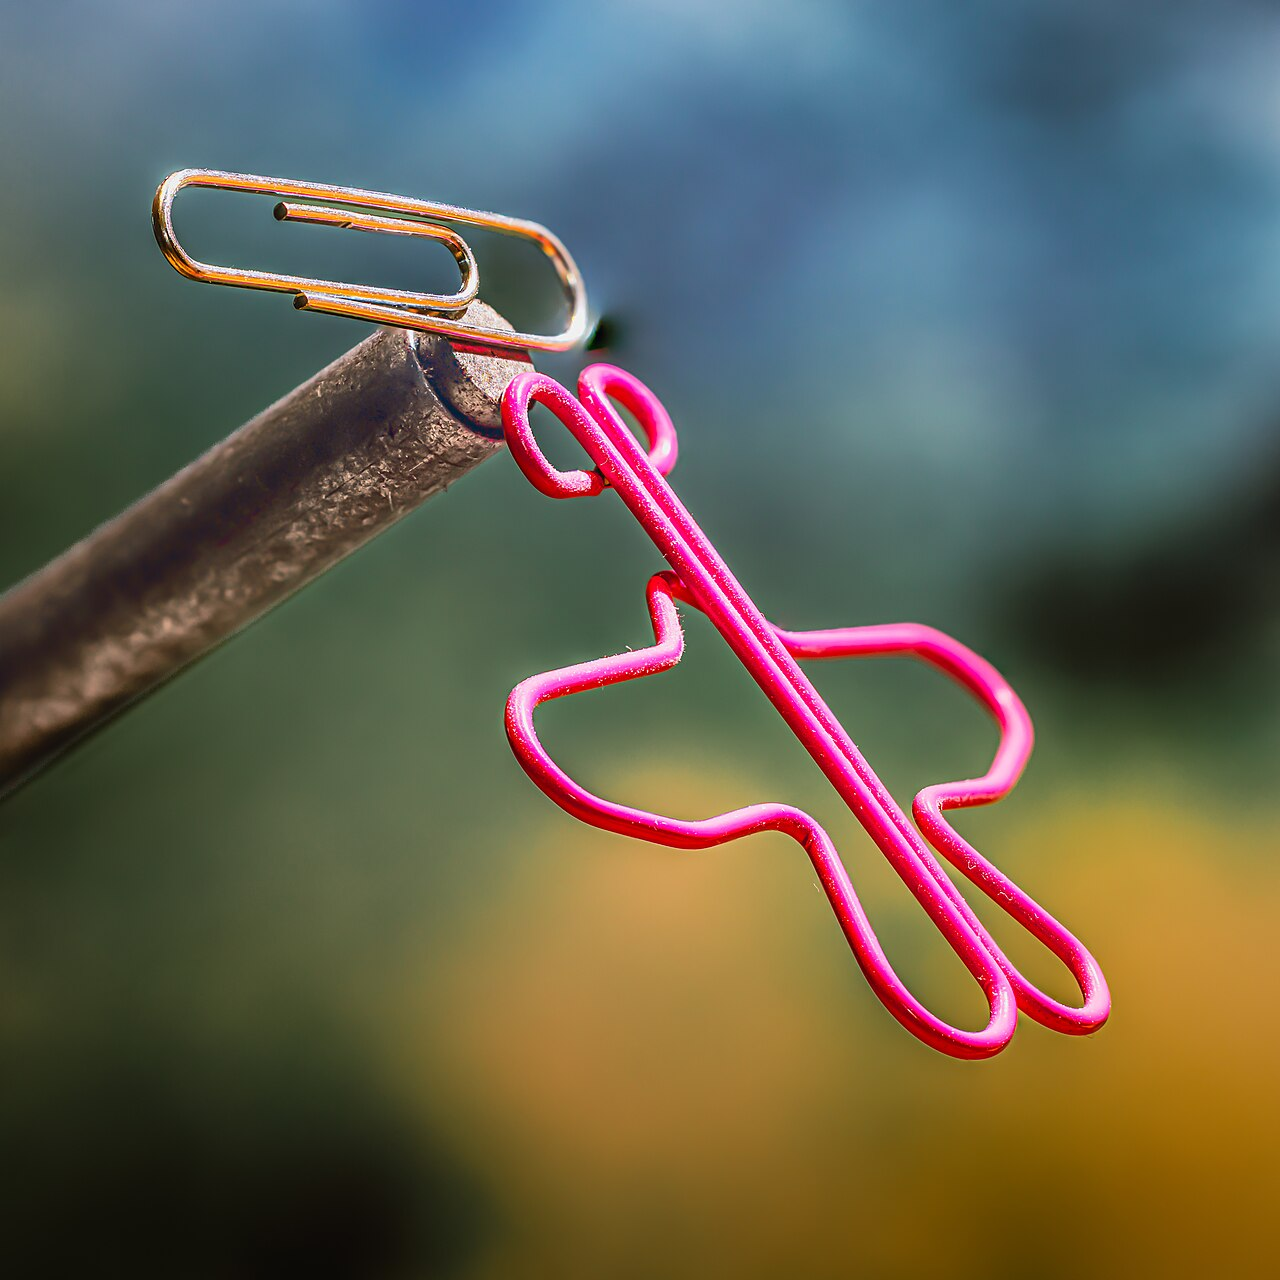
\includegraphics[width=0.5\linewidth]{images/book1/magnet-paperclips.jpg}

{\small 磁铁的实际应用：回形针挂在一根被磁化的棒子的
顶端。粉色回形针外面包着塑料 --- 拉力
直接穿过了它的外层。\emph{Photo: Donald Olszewski,
CC BY 4.0.}}
\end{omfigure}

\begin{method}[磁铁钓鱼]\label{met:g1:magnets:fishing}
这是一个两人游戏，也是检验“够得着”范围的公平试验：
\begin{enumerate}
  \item 把磁铁系在细绳上 --- 这就是“鱼竿”；
  \item 把回形针撒在地板上 --- 这些就是“鱼”；
  \item 把磁铁从一枚回形针的正上方慢慢放下；
  \item 回形针跳起吸向磁铁的那一时刻，立即停止下放。
\end{enumerate}
只有磁铁靠得很近时，回形针才会跳起：磁铁附近的
拉力很强，离得稍远就迅速减弱。
\end{method}

\section{两块磁铁靠在一起}

\begin{example}[试一试：是吸引还是排斥？]\label{ex:g1:magnets:twomagnets}
两手各拿一块磁铁，把它们的一端慢慢靠近，
有时它们会互相跳过去，“啪”的一声吸在一起。
现在把其中一块磁铁调个头，换另一端朝前，再让它们靠近，
这一次你会感到柔和、有弹性的\emph{排斥}力 ---
磁铁不肯相碰，仿佛两者之间夹着一个看不见的软垫，
它们之间。同样两块磁铁，一种摆法相互吸引，调个头就相互排斥。
\end{example}

\begin{omfigure}
\begin{tikzpicture}[scale=0.85]
  % different colors face each other: attraction
  \draw[thick, fill=red!70] (0,1.1) rectangle (0.9,1.8);
  \draw[thick, fill=blue!60] (0.9,1.1) rectangle (1.8,1.8);
  \draw[thick, fill=red!70] (3.4,1.1) rectangle (4.3,1.8);
  \draw[thick, fill=blue!60] (4.3,1.1) rectangle (5.2,1.8);
  \draw[-Stealth, very thick] (1.95,1.45) -- (2.5,1.45);
  \draw[-Stealth, very thick] (3.25,1.45) -- (2.7,1.45);
  \node[below, font=\small, align=center] at (2.6,0.85)
    {异色端相对：\\它们跳到一起};
  % same colors face each other: repulsion
  \draw[thick, fill=red!70] (7.0,1.1) rectangle (7.9,1.8);
  \draw[thick, fill=blue!60] (7.9,1.1) rectangle (8.8,1.8);
  \draw[thick, fill=blue!60] (10.4,1.1) rectangle (11.3,1.8);
  \draw[thick, fill=red!70] (11.3,1.1) rectangle (12.2,1.8);
  \draw[-Stealth, very thick] (6.85,1.45) -- (6.3,1.45);
  \draw[-Stealth, very thick] (12.35,1.45) -- (12.9,1.45);
  \node[below, font=\small, align=center] at (9.6,0.85)
    {同色端相对：\\它们互相推开};
\end{tikzpicture}

{\small 两组磁铁，各有颜色不同的两端。当两个
\emph{不同}颜色的一端相对时，磁铁互相吸在一起；
把其中一块调个头，让\emph{相同}的一端相对，它们就彼此
推开。}
\end{omfigure}

\begin{remark}[磁铁的两端]\label{rem:g1:magnets:ends}
所以磁铁的两端并不相同，即使看起来很相似！
每块磁铁都有两个不同的端，吸与斥取决于
\emph{哪一端}相遇。也可以用回形针来试一试：
回形针聚集在条形磁铁的两端，中间部分几乎不吸。
这两个特殊的端有各自的名字，还有一项著名的任务 ---
为远行的旅人指引方向 --- 不过这个故事要等到
本书后面的年级再讲。
\end{remark}

\section{练习}

\begin{exercise}[$\star$]\label{exo:g1:magnets:1}
将下列物品分为“磁铁会吸住”和“磁铁不理会”两类：
一枚钉子；\ 一个软木塞；\ 一枚回形针；\ 一只塑料鸭子；\ 一把钢勺；\ 一
张纸。
\end{exercise}

\begin{exercise}[$\star$]\label{exo:g1:magnets:2}
磁铁喜欢哪一类东西？请说出两种磁铁始终不理会的
金属或材料。
\end{exercise}

\begin{exercise}[$\star$]\label{exo:g1:magnets:3}
一张图画用磁铁压在冰箱门上。磁铁和门
之间夹着什么？这说明磁铁的拉力
有怎样的特点？
\end{exercise}

\begin{exercise}[$\star$]\label{exo:g1:magnets:4}
一枚回形针掉进一杯装满水的杯子里。怎样才能
用磁铁把它取出来，而手指不沾水？
\end{exercise}

\begin{exercise}[$\star$]\label{exo:g1:magnets:5}
在\cref{met:g1:magnets:fishing}中的磁铁钓鱼游戏里，回形针
只有磁铁靠近时才会跳起。这说明在离磁铁
较远的地方，拉力有什么特点？
\end{exercise}

\begin{exercise}[$\star$]\label{exo:g1:magnets:6}
把两块磁铁一端对一端靠近，它们会吸在一起。只需做一个
简单的动作，同样两块磁铁就会改为相互推开？
\end{exercise}

\begin{exercise}[$\star$]\label{exo:g1:magnets:7}
回形针在条形磁铁上聚集在哪里：中间还是
两端？这说明磁铁在哪里最强？
\end{exercise}

\begin{exercise}[$\star$]\label{exo:g1:magnets:8}
请说出一点：磁铁与你用手移动玩具有相似之处；再说出一点
它们完全不同。（想一想
\cref{rem:g1:magnets:notouch}。）
\end{exercise}

\begin{exercise}[$\star\star$]\label{exo:g1:magnets:9}
汤姆说：“磁铁会吸引所有金属制成的东西。”请设计一个
小实验，用一枚硬币、一枚钉子和厨房锡纸，检验汤姆的
这句话，说明会出现什么现象，并改正他的句子。
\end{exercise}
